\documentclass{article}
\usepackage[utf8]{inputenc}
\usepackage[T1]{fontenc}
\usepackage{graphicx}
\usepackage{hyperref}
\usepackage{geometry}
\geometry{margin=1in}

\title{Britannica Volume 149981670 Row 1344}
\date{Encyclopaedia Britannica (1771)}

\begin{document}
\maketitle

\section*{Historical source}
\textbf{Entry ID:} \texttt{entry-britannica-volume-149981670-row-1344-1344} \\
\textbf{Volume ID:} 149981670 \\
\textbf{Character Count:} 6463

\subsection*{Extracted Text}
H O R [ 664 ] H O R

Horfs

be totally cled up, or the cranium in that part not be
to hard as the rest for four years after. This is made
refs is found to be incredied upon the child’s catching
cold. When the differdit continuer long, it is repu-
ted a drop of webendo and flour life, in this case
it is usual to rub the head now and then with warm
rum or bowled, mixed with the white one leg against
pain oil. Sometimes the different suffer from a col-
lection of waters in the head called an \_hydrosepholes\_.

\_Since Horse\_ See StylLON.

\_Horas Tall.\_ Se Egyptian and EPIRRA.

\_Horas Path.\_ See Hippocrates.

\_Wars Horas.\_ The proper rules for choosing a horfe
for carrier in war, are neither he should be tall in fiat-
ture, with a county break, and out-fwelling forecechs
His eye should be bright and parbling, and the white
part of it covered by the eye brow. The cats should
be final, thin, there, and pinkking , or if longer, the
should be manhole with rafa, and well carried. The
neck should be deep, and the breath large and fewling.
The ribs bending, the either bound and flagging, and
the buttons round and fall. The tail though be high
and broad, neither too thick nor too thin; the thigh
wellings; the leg broad and like, and the pallon them.
When fush a horse he chodey, he must be kept high de-
ring the time of his teaching, that he may be full of
vigore. His bondmilt be free to any good and clean out
or two parts of cats and one part, feeding our prefer,
well dried and hardened. The quantity should be half
a peck in the oneming, and the have quantity at now
and in the evening. Upon his cutting days he is to be
drifted, between five and the less than morning, and
el at times or rights, to the evening he is to be dificult
at four, and watered about five, and he mull always
have provided given him into after evening; he must be
littered about sight, and then muff the food gli-
ven him for all night. The night before he is ridden
all last hay is to be has a way about nine of checks, and
he mull have a handful or two of cats also took four
the morning; when he has eaten theirly leis to do
turned upon the traffic, and indeed very well with dry
wilps. Then fadidlek, and made it for his exercise.
When he has performed this, is to the boven
freezing into the thlile, and tribbed down with dry
wifps. When this has been done, the fiddle is to be
tant and, and he is to be crbbedded down with the clothes
the houling cloth is then to be had on) and the double
being again kid on, he is to be walked gently about
till thoroughly cool. After that, he mull fixed with
out meat two or three hours, then he mull be fed, yet
in the afternoon he is to be rubbed and dreified as be-
fore, and waccent in the ritual menor.

\_Horas Wow, in\_ natural history, a species of fly-
worm called \_also lead\_, produced e eggs deposited by a
two-wing fly of the flop and line of the humble
be in the intestines of horses. See Boryss.

\_Rose Horns, in another.\_ Se El Hyporomans.

Horas is alo old in the military language, to cees
pets the country or the body of folders who feevo on
horfeback.

The horfe includes horfe guards, hoeře genaudlers,
and troopers. Dragoons are allo frequently compro-
hended under this name, though they fight on foot:
of these there are now 18 regiments ) believes re-
No 157.

ments of dragon-quards infed in 1682. See Gra-
Roors, Dragoons), and Guaxan.

\_Molter of the Horns.\_ See Marxer.

\_Light Horns\_ are regiments of cavalry mounted on
light fruit horches, which may see final and lightly ac-
cutout. They were first infed in 1757). The deno-
manism and hence, chat anxietly they were lightly
armed, in comparison of the royal guards, which were
arned at all points.

\_Hongangna Horns.\_ Se El Dorass

Horse is alo often used its various arts and manu-
factories, for fomething that helps to fuflain their
work from the ground, for the more commodious
working at it.

The horf died by transers and filmmers, alfo called
the Ig, ira piece of wood cut hollow and rounds,
four or five feet long, and placed slippers upon which
they per their dens et get of the dirty hair, flesh,\&.

Horas is alo did not in empery for a price of wood
pointed across two other perpendicular ones, to fulain
the boards, phunks, so, which make bridges over-final
rivers and no divers other conditions.

Horas, in tea language, is the name of a rope reach-
ing from the middle of a yards in its ceremony or what
called the \_predecessor\_, and depending about two or
three feet under the yard, for the failors to tread upon
which they are holding, resting, holding the fails, op-
ing and the fluidizing fall bombs, etc. It orders, therefore, to keep the horfe more parallel to the yard, it is
usually fupdated to it at a proper distance, by certain
roppes called dirtrops, which hang about two feet under
the yard, having my eye in their lower ends through
which the horfe place.

Horos is alo a thick rope, extended in a perpendli-
line direction near east four or after field at each if,
the poprue of boiling or extending force fall upon it.
When it is fixed before a mafts, it is calculated for the
use of a fall called the former folkl, whole you'd being ex-
tached to the horfe, by means of a rareclier or bull's
eye, which chips and down occasionally, is retained
in a likely position where when the fail is fet, or
whilst it is holding or lowering. When the horfe is
places itself or behind a mafts, it is intended for the
crystal of a few, and is according to party fixed
in this position, except in those floors of war which oc-
refundally slither the form of flows, in order to dec-
ners the enemy.

Horos is alo a cant name introduced into the mas-
agement of batteries, the chance or benefit of a
ticket or number for one or more days, soon consider
tion, if it be drawn a prize within the time ceremonies
for, of returning to the false or undrawn tickets—To
determine the value of a horfe ) multiply the amount
of the prizes in the lottery by the time the horfe is ha-
red for, and from the produce fabricated the amount of
the number of prizes by the value of an undrawn tic-
ket into the time of the horfe., the remaining being
divided by the number of tickets onto the whole time of
drawing, the quotient is the value of the horfe. See
Boryss.

\_Horas-Bread.\_ See Barxad.

\_Horas-Dang\_ in gardening, is o great ufc in ma-
king hot-beds, for the rafting all sorts of early crops
as fishing, cucumbers melons, afparagus, \&c, for
which

\subsection*{Matched Wikipedia Article}
\textbf{Title:} Editor-in-chief of the Encyclopædia Britannica \\
\textbf{Page ID:} 78413092 \\
\textbf{Revision ID:} 1351079103 \\
\textbf{URL:} \url{https://en.wikipedia.org/wiki/Editor-in-chief\_of\_the\_Encyclop\%C3\%A6dia\_Britannica}


\section*{Source record}
\begin{itemize}
\item \textbf{Dataset:} \texttt{NationalLibraryOfScotland/encyclopaedia\_britannica\_illustrated}
\item \textbf{Dataset Revision:} \texttt{309f765b1ecc83e0a7f7762e44b4a927a7555443}
\item \textbf{Page ID:} \texttt{britannica:309f765b1ecc83e0a7f7762e44b4a927a7555443:train:1344} \\
  \textbf{Filename:} \texttt{page-1344-b5c2505d4784.jpg} \\
  \textbf{Row Index:} 1344 \\
  \textbf{SHA256:} \texttt{b5c2505d4784ce9e...}
\end{itemize}

\begin{figure}[h]
\centering
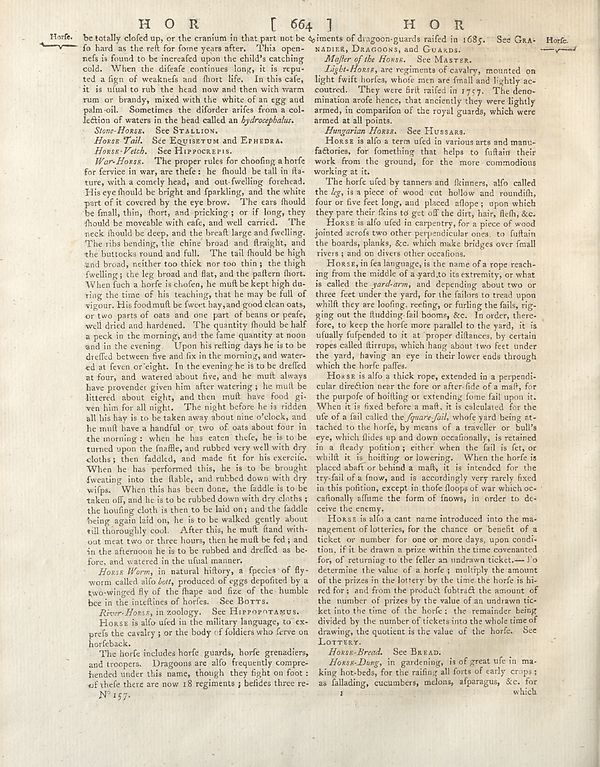
\includegraphics[width=0.85\textwidth]{../scans/page-1344-b5c2505d4784.jpg}
\caption*{Source scan: \texttt{page-1344-b5c2505d4784.jpg}}
\end{figure}

\end{document}
